\IEEEraisesectionheading{\section{Introduction}\label{sec:introduction}}
\nocite{ProjectCode}
The objective of the project \glqq Towards real-time physics in a 2D survival-based game\grqq{} is
a comprehensive restructuring and improvement of the original game \glqq Surviving Sarntal\grqq{}.
This comprises three major work packages: software engineering, development of real-time physics and game engineering.

% Software engineering part: 
The first part of the project focuses on improving the code by adherence to software engineering principles.
This includes extensive refactoring of the original code base, designing a new and maintainable software architecture,
establishing protocols for development, testing and clean code as well as creating a platform for detailed documentation for users and developers.
The project's continuous progress was ensured by applying Scrum principles and structuring it in sprints \cite{scrum}.
% We carried out a total of three sprints, whereby at the beginning of each sprint we defined the objectives at the end of the sprint
% and the issues to be dealt with. On a weekly basis, a meeting was held with our supervisor.
% During these meetings, the current progress regarding the project timeline, ideas and challenges occurring in development were discussed.
% Furthermore, two time slots were determined each week for a brief discussion of each team member's current work.
% The GitLab \glqq Issues\grqq{} were used to determine feasible work packages, which then could be assigned to one team member.

% Real time physics: 
The primary goal of the development phase is the enhancement of the real-time physics,
which involves the implementation of realistic 2D physics without compromising real-time performance.
This was accomplished by decoupling the physics simulation rate from the frame rate.
Furthermore, the project includes the development and implementation of improved models and algorithms
for interaction between game elements such as collision detection and handling.

% Game engineering
Moreover, the project contributes to the enhancement of the game design as a whole.
A number of new elements have been implemented, such as configurable 2D spline-based terrain generation, 
new items with improved functionality, new rock generation, increasing difficulty and updated audio and graphics.

% "Conclusion of the Introduction" 
In essence, the project was developed in accordance with the vision of creating an enhanced version of the game \glqq Surviving Sarntal\grqq{}
that would offer users a realistic physics simulation, engaging gameplay, and aesthetically pleasing visuals as well as creating a maintainable code base.
The code for the game is available as a git repository here \cite{ProjectCode} and it is open source under an MIT license.

\subsection{The Game}
The general goal of the game is for the hiker to survive as long as possible and climb as high as possible. 
The player is chased by a monster and needs to evade rocks that roll down the mountain. 
Moreover, the player may collect items that give the hiker additional benefits like restoring health and adding a protective shield. 
A comprehensive guide to the controls can be found in the project documentation \cite{ProjectWiki} and at the start of the game under the menu "Instructions". 

\subsection{Transformation of the original game}
The original game \glqq Surviving Sarntal\grqq{} was created within a few days at the \glqq Ferienakademie 2023\grqq{}.
In this project, we refactor the original game in a significant way. 

\subsubsection{ECS vs. OOP}
The original game is based on the Entity-Component-System (ECS) framework flecs \cite{flecs_library}.
As a team, we decided to alter the project's fundamental architecture by shifting from ECS
to an object-oriented programming (OOP) approach.
Given our familiarity with OOP, we came to the conclusion that transitioning from ECS to OOP
would allow us to create a code base that could be easily comprehended, expanded and maintained.

\subsubsection{Transformation of Graphics}
During the development process of the new version of the game, we decided that a complete rework of the game's graphics was necessary.
New and creative graphical elements were created for all aspects of the game, including the entities, terrain, and background, and were integrated into the rendering phase of the game.
Screenshots of the old game can be seen in fig. \ref{fig:old_game} and of the new game in fig. \ref{fig:new_game}.

\begin{figure}[h!]
    \centering
    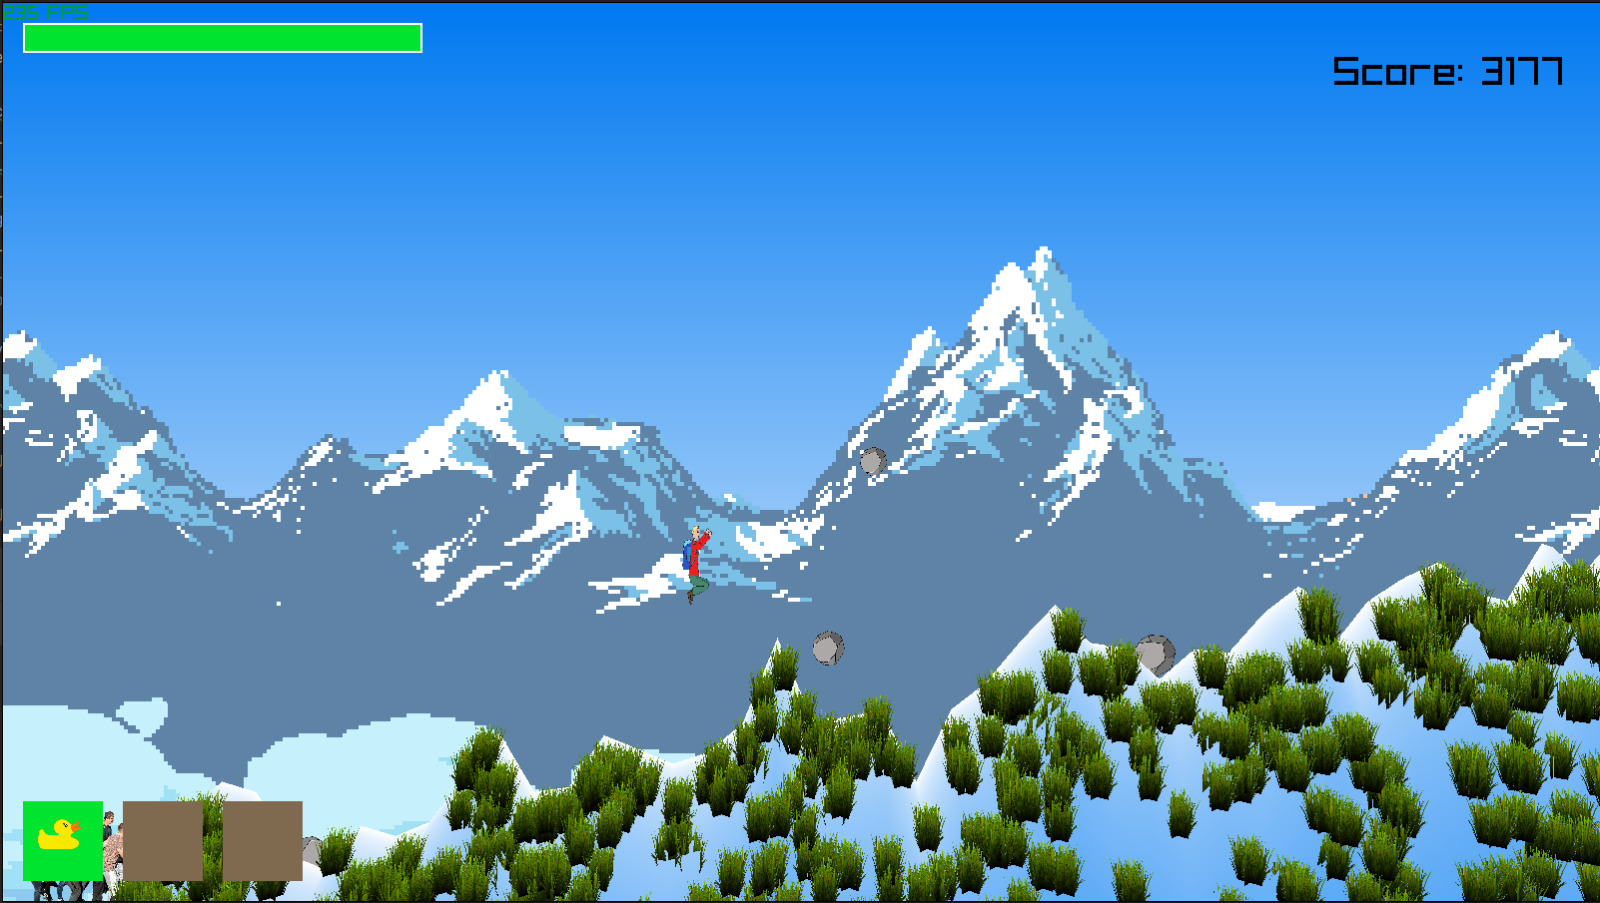
\includegraphics[width=0.45\textwidth]{figures/old_game.jpeg}
    \caption{Screenshot of the original game graphics.}
    \label{fig:old_game}
  \end{figure}

\begin{figure}[h!]
    \centering
    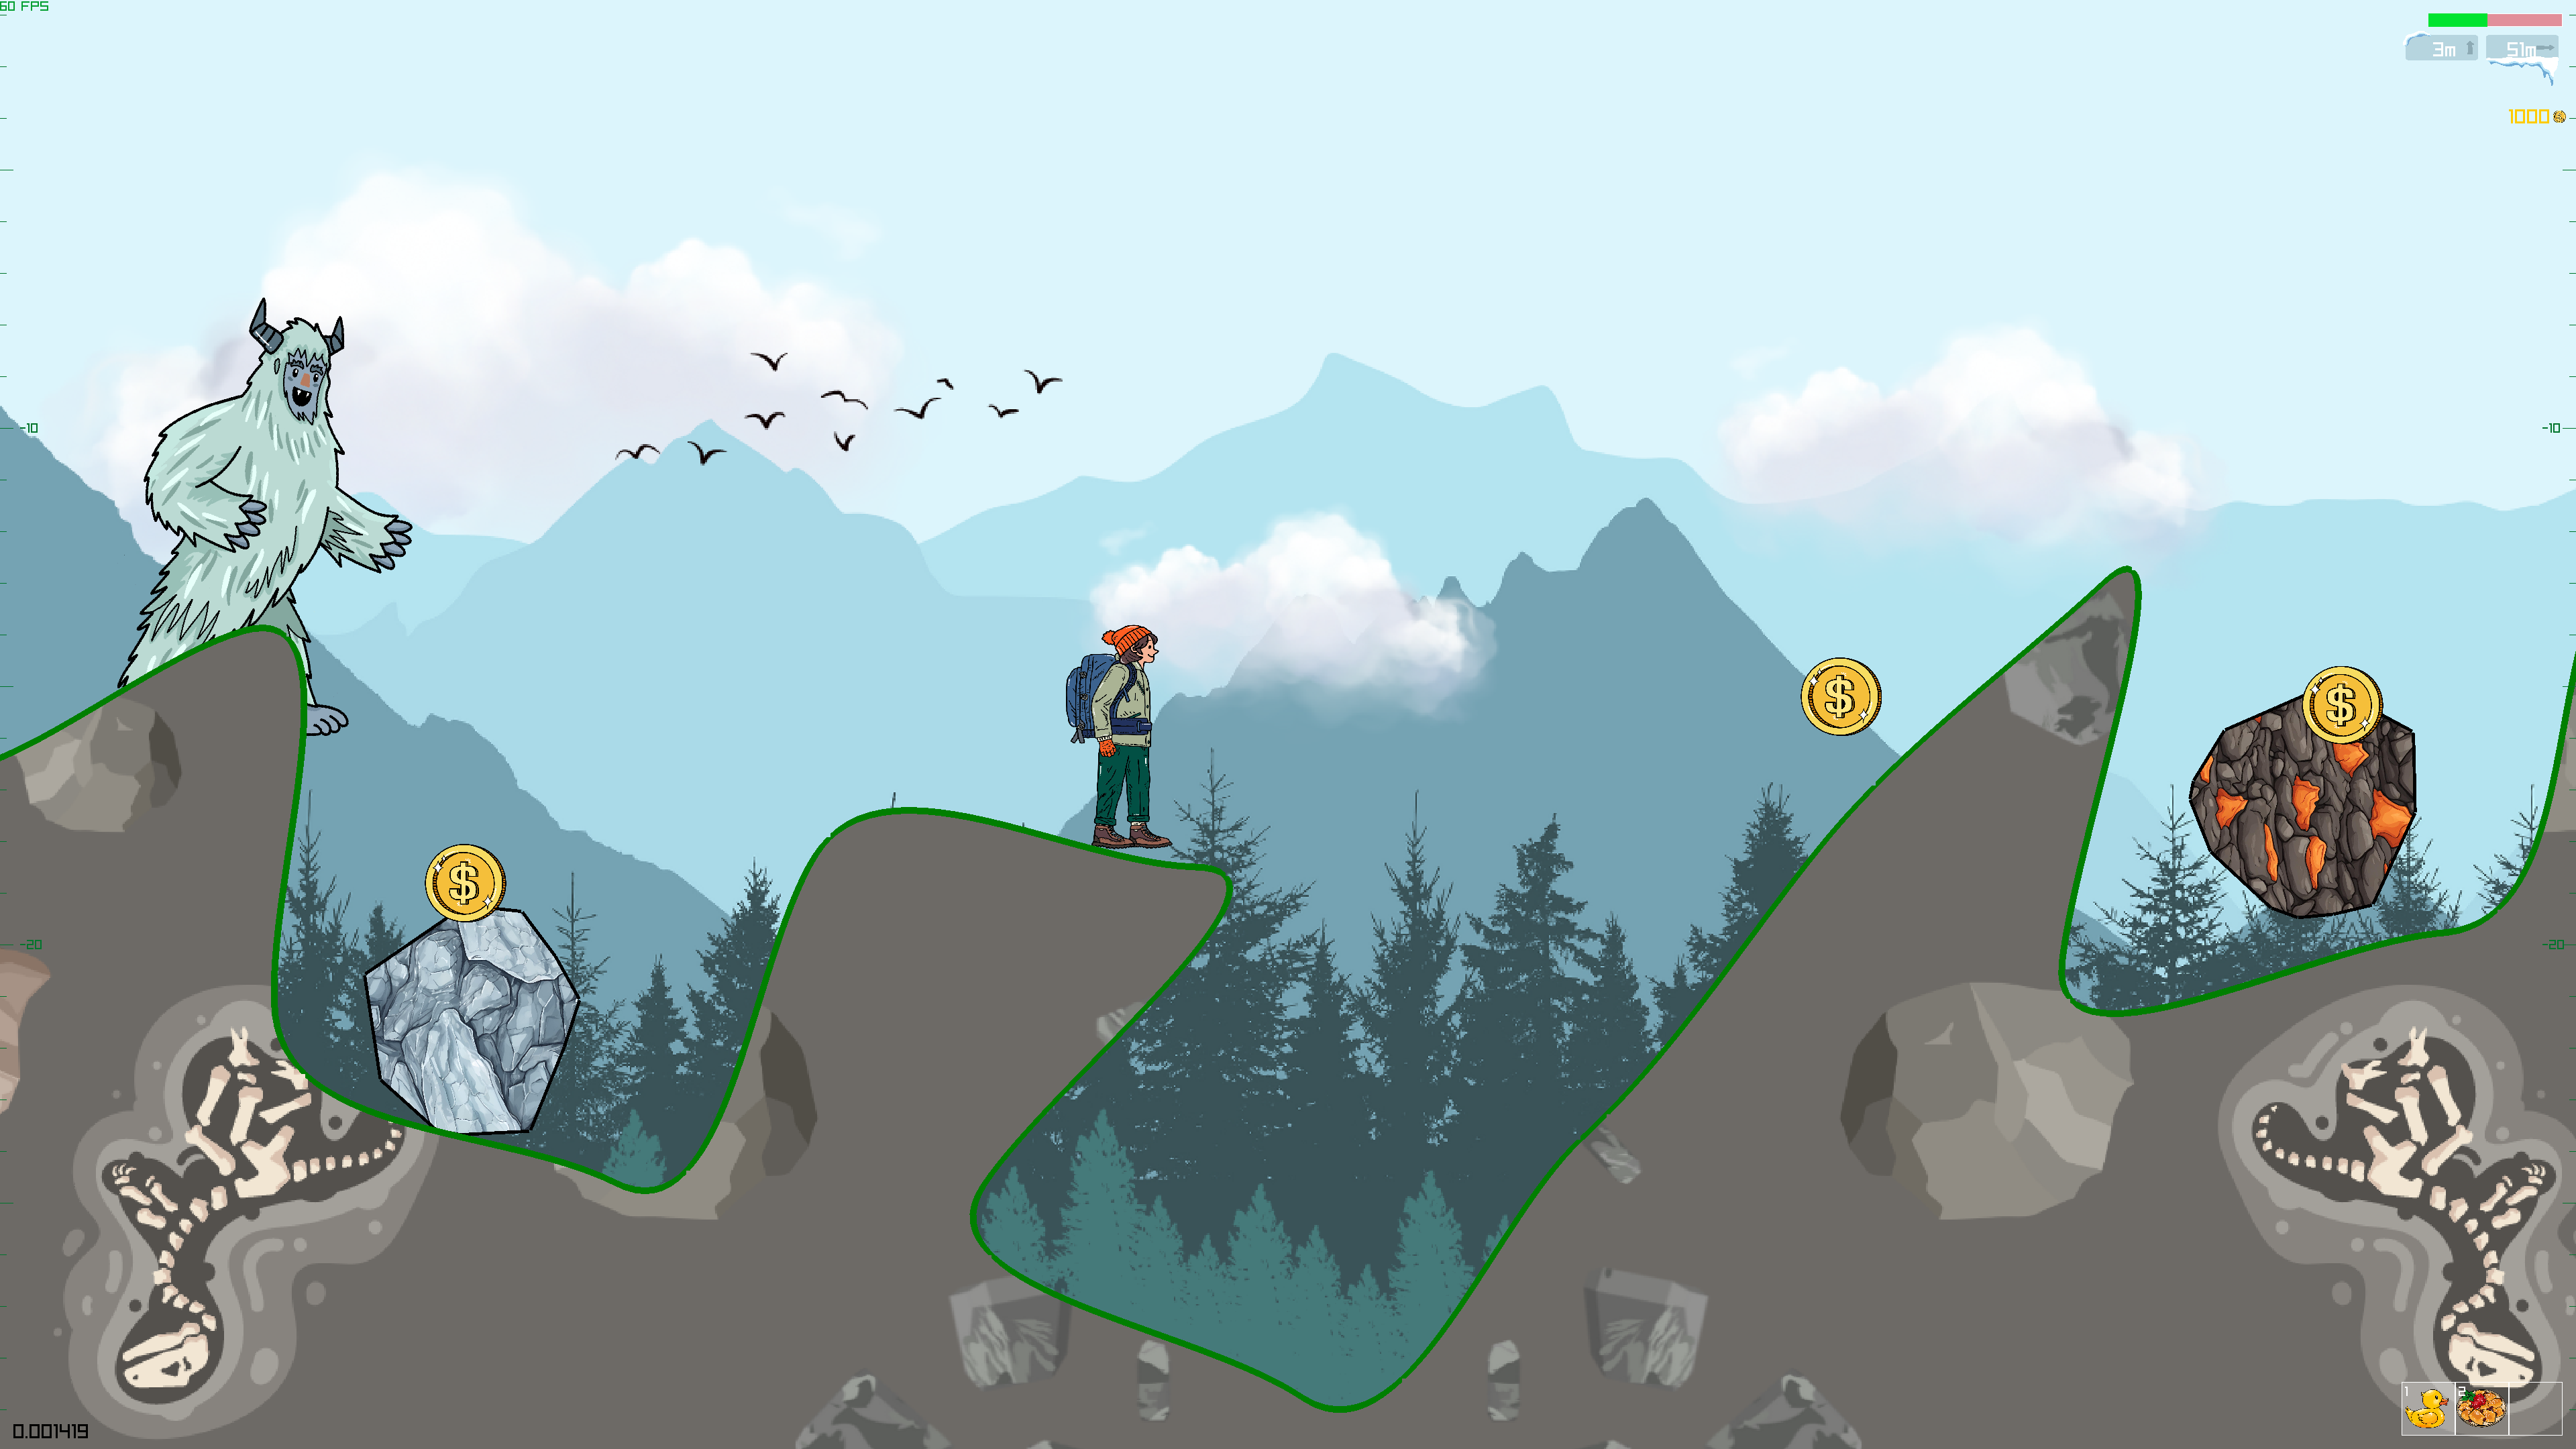
\includegraphics[width=0.45\textwidth]{figures/new_game.png}
    \caption{Screenshot of the renewed game graphics.}
    \label{fig:new_game}
  \end{figure}

\subsubsection{Addition of a game menu}
As a new feature we include a game menu.
A start menu is shown once the game has been initiated, which allows the user to access instructions and controls, and to start the gameplay.
An end screen appears after the hiker has died, which enables them to start another round of gameplay. 
We also add a pause screen, which gives the user the options to go back to the main menu or continue the game.

\subsubsection{Modular Architecture}
As part of the software engineering work package of the project we designed a modular game architecture that provides several key benefits:
\begin{itemize}
    \item \textbf{Ease of Maintenance:} Since components such as rendering, physics, and spawning are isolated from each other, it is easier to modify, debug, or upgrade parts of the game without introducing side effects.
    \item \textbf{Maintainability:} New features or game elements (e.g., new items, enemies, or gameplay mechanics) can be added by extending existing systems without requiring significant changes to the core architecture.
    \item \textbf{Testing and Debugging:} We add multiple features for developers, like a debug view seen in fig. \ref{fig:debug_mode} and a developer mode of the game that allows the running of predefined test cases. 
    \item \textbf{New terrain:} We extend our modular design to the terrain, by creating a completely new class structure that allows for different terrains with different features to be added.
\end{itemize}
This modular structure enables the development team to build complex systems in a more controlled and efficient manner, leading to a highly extensible and maintainable game.